% DEC-066 ablation and closure results (inserted by IEEE39_DEC066_results_draft.tex, subsection "Contribution of the overshoot term").
% Numbers come from artifacts/IEEE39_DEC066_T4*.csv, T4e, T5*_observed.csv, T5b, T6, T7*, T8; tables are generated (IEEE39_DEC066_ablation_tables.tex, IEEE39_DEC066_closure_tables.tex).
% 34 time-domain simulations (ANDES RMS/phasor, controller B5', OC1); hypotheses and predictions were sealed before each lot (IEEE39_DEC066_E1a/E1b/E2/F2/F3/F4/F5_plan.json).
% Generated by dec066_abl_latex.py from IEEE39_DEC066_T*.csv (DEC-066). Do not edit by hand.
\begin{table*}[t]
\centering\footnotesize
\caption{The five preventive designs (OC1; same 12 design events, objective, solver and settings; none certified optimal). Margins are predicted minimum Pmax margins over the design events without $\varepsilon$ margins: ``grid'' uses the M3 excursion on the 195~s grid, ``dense'' adds the 0--50~ms evaluation. Design A was optimised with M0 as an additional seed, B--E from M3; the KKT residual of B (0.598) shows that it is not a converged point.}
\label{tab:ablation_designs}
\resizebox{\linewidth}{!}{\begin{tabular}{llrrrrrrlrr}
\toprule
Design & Status & $J$ & $\sum|\Delta P|$ vs case (MW) & vs A (MW) & KKT & margin grid (pu) & margin dense (pu) & limiting & Plant eval. & Time (s) \\
\midrule
A (M3) & feas.\ pred. & 1.6815 & 55.7 & 0.0 & 0.062 & 0.0020 & -0.0150 & SG31 b8P\_S3 & 440 & 1489 \\
B (+dense) & feas.\ pred. & 1.7055 & 57.2 & 2.2 & 0.598 & 0.0020 & 0.0020 & SG31 b8P\_S3 & 516 & 1304 \\
C (+dense$+\varepsilon_{OS}$) & feas.\ pred. & 1.7073 & 57.2 & 2.4 & 0.060 & 0.0024 & 0.0024 & SG31 b8P\_S3 & 438 & 1065 \\
D (M3+OS) & feas.\ pred. & 1.7591 & 61.2 & 6.8 & 0.058 & 0.0133 & 0.0133 & GFM36 b23P\_S3 & 394 & 664 \\
E ($U_{D8}$ only) & feas.\ pred. & 1.7309 & 58.8 & 3.5 & 0.062 & 0.0129 & -0.0041 & SG31 b8P\_S3 & 395 & 925 \\
\bottomrule
\end{tabular}}
\end{table*}

\begin{table*}[t]
\centering\footnotesize
\caption{Observed minimum Pmax margin of delivered power against the margin registered before the simulations (B5$'$, OC1, 17 runs). Class by rule M3V-1 (band $\pm U_{D8}=0.0109$~pu); ``Viol.'' flags $m<0$ even when it lies inside the band (INDET.). Error: observed $-$ predicted (positive: conservative). Duration is the integral of the below-limit indicator over stored samples (local step 0.24~ms), hence approximate. $t_{\rm pk}$ is the first stored sample of the minimum. The last three columns are the observed margin in 50~ms--10~s (pu), the COI frequency nadir (Hz) and the minimum bus voltage (pu).}
\label{tab:ablation_obs}
\resizebox{\linewidth}{!}{\begin{tabular}{llrrrlcrrlrrrr}
\toprule
Event & Design & Pred. & Obs. & Error & Class & Viol. & Excess & Dur. (ms) & Unit & $t_{\rm pk}$ (ms) & $m_{50\rm ms-10s}$ & $f_{\rm nadir}$ & $V_{\min}$ \\
\midrule
b15 S3 & A & -0.0070 & -0.0068 & 0.0002 & INDET. & yes & 0.0068 & 0.73 & SG33 & 2.44 & 0.101 & 59.964 & 0.971 \\
b15 S3 & D & 0.0080 & 0.0081 & 0.0002 & INDET. & no & 0.0000 & 0.00 & SG33 & 2.44 & 0.128 & 59.964 & 0.971 \\
b21 S2 & A & 0.0907 & 0.0909 & 0.0002 & SAFE & no & 0.0000 & 0.00 & SG33 & 2.44 & 0.131 & 59.977 & 0.975 \\
b21 S2 & D & 0.1057 & 0.1059 & 0.0002 & SAFE & no & 0.0000 & 0.00 & SG33 & 2.44 & 0.158 & 59.977 & 0.975 \\
b21 S3 & A & -0.0113 & -0.0110 & 0.0003 & UNSAFE & yes & 0.0110 & 0.98 & SG33 & 2.44 & 0.099 & 59.964 & 0.972 \\
b21 S3 & B & -0.0076 & -0.0072 & 0.0004 & INDET. & yes & 0.0072 & 0.73 & SG33 & 2.44 & 0.115 & 59.964 & 0.972 \\
b21 S3 & D & 0.0037 & 0.0040 & 0.0003 & INDET. & no & 0.0000 & 0.00 & SG33 & 2.44 & 0.126 & 59.964 & 0.972 \\
b21 S3 & E & -0.0097 & -0.0094 & 0.0004 & INDET. & yes & 0.0094 & 0.98 & SG33 & 2.44 & 0.110 & 59.964 & 0.972 \\
b23 S3 & A & 0.0000 & 0.0006 & 0.0006 & INDET. & no & 0.0000 & 0.00 & SG33 & 2.44 & 0.064 & 59.965 & 0.973 \\
b23 S3 & D & 0.0133 & 0.0156 & 0.0024 & SAFE & no & 0.0000 & 0.00 & SG33 & 2.44 & 0.075 & 59.965 & 0.972 \\
b31 S2 & A & -0.1279 & -0.1278 & 0.0002 & UNSAFE & yes & 0.1278 & 57.98 & SG31 & 1.95 & -0.010 & 59.977 & 0.977 \\
b31 S2 & D & -0.0994 & -0.0992 & 0.0002 & UNSAFE & yes & 0.0992 & 36.50 & SG31 & 1.95 & 0.019 & 59.977 & 0.977 \\
b8 S3 & A & -0.0150 & -0.0148 & 0.0002 & UNSAFE & yes & 0.0148 & 1.46 & SG31 & 2.20 & 0.083 & 59.965 & 0.970 \\
b8 S3 & B & 0.0020 & 0.0023 & 0.0003 & INDET. & no & 0.0000 & 0.00 & SG31 & 2.20 & 0.100 & 59.965 & 0.970 \\
b8 S3 & C & 0.0024 & 0.0027 & 0.0003 & INDET. & no & 0.0000 & 0.00 & SG31 & 2.20 & 0.100 & 59.965 & 0.970 \\
b8 S3 & D & 0.0133 & 0.0136 & 0.0003 & SAFE & no & 0.0000 & 0.00 & SG31 & 2.20 & 0.111 & 59.965 & 0.970 \\
b8 S3 & E & -0.0041 & -0.0038 & 0.0003 & INDET. & yes & 0.0038 & 0.73 & SG31 & 2.20 & 0.093 & 59.965 & 0.970 \\
\bottomrule
\end{tabular}}
\end{table*}

\begin{table}[t]
\centering\footnotesize
\caption{Marginal contrasts between designs: change in the observed minimum Pmax margin (pu) and in the design effort. The five designs are a directed set, not a factorial: the contrasts $B-A$ (dense), $C-B$ ($\varepsilon_{OS}$), $D-C$ ($U_{D8}$ given dense and $\varepsilon_{OS}$), $E-A$ ($U_{D8}$ alone) and $D-E$ (dense and $\varepsilon_{OS}$ given $U_{D8}$) are not additive and interactions are not identified. ``Viol.'' columns: $m<0$ in the first / second design of the pair. The effort difference is a design-level quantity (MW, $J$), identical for all events.}
\label{tab:ablation_contrasts}
\resizebox{\linewidth}{!}{\begin{tabular}{llllccrr}
\toprule
Event & Contrast & Component & $\Delta m_{\rm obs}$ & Viol. (1st) & Viol. (2nd) & $\Delta\sum|\Delta P|$ (MW) & $\Delta J$ \\
\midrule
b8 S3 & B-A & dense & 0.0170 & yes & no & 1.46 & 0.0240 \\
b8 S3 & C-B & eps\_OS & 0.0004 & no & no & 0.07 & 0.0018 \\
b8 S3 & D-C & U\_D8 | dense+eps\_OS & 0.0109 & no & no & 3.96 & 0.0519 \\
b8 S3 & E-A & U\_D8 alone & 0.0109 & yes & yes & 3.13 & 0.0494 \\
b8 S3 & D-E & dense+eps\_OS | U\_D8 & 0.0174 & yes & no & 2.37 & 0.0283 \\
b8 S3 & D-A & full OS & 0.0283 & yes & no & 5.50 & 0.0777 \\
b21 S3 & B-A & dense & 0.0037 & yes & yes & 1.46 & 0.0240 \\
b21 S3 & E-A & U\_D8 alone & 0.0016 & yes & yes & 3.13 & 0.0494 \\
b21 S3 & D-E & dense+eps\_OS | U\_D8 & 0.0134 & yes & no & 2.37 & 0.0283 \\
b21 S3 & D-A & full OS & 0.0150 & yes & no & 5.50 & 0.0777 \\
b15 S3 & D-A & full OS & 0.0150 & yes & no & 5.50 & 0.0777 \\
b23 S3 & D-A & full OS & 0.0150 & no & no & 5.50 & 0.0777 \\
\bottomrule
\end{tabular}}
\end{table}

% Generated by dec066_close_latex.py from IEEE39_DEC066_T4e/T7/T8 CSV (DEC-066). Do not edit by hand.
\begin{table*}[t]
\centering\footnotesize
\caption{Designs at (approximately) equal redispatch effort: E and DQ1 at about 58.7~MW, D and EQ1 at about 61.2~MW (sum of $|\Delta P|$ against the case dispatch; equal redispatch is not equal economic cost, see $J$). Predicted: minimum external margin over the 12 design events (grid+dense excursion, no $\varepsilon$) and number of the 27 valid design and evaluation events with negative predicted margin. Observed: minimum Pmax margin 0--10~s in the time-domain simulation (pu; ``viol.'' = $m<0$) and pre-event headroom of the limiting unit at the two events simulated for all five designs (bus 8: SG31; bus 21: SG33).}
\label{tab:equaleffort}
\resizebox{\linewidth}{!}{\begin{tabular}{lrrrrrrrr}
\toprule
Design & $\sum|\Delta P|$ (MW) & $J$ & pred. min margin & events $m<0$ & obs. b8 S3 & headroom SG31 & obs. b21 S3 & headroom SG33 \\
\midrule
A (M3) & 55.7 & 1.6815 & -0.0150 & 6/27 & -0.0148 (viol.) & 0.191 & -0.0110 (viol.) & 0.294 \\
E ($U$ only, 0.0109) & 58.8 & 1.7309 & -0.0041 & 6/27 & -0.0038 (viol.) & 0.202 & -0.0094 (viol.) & 0.295 \\
DQ1 (dense$+\varepsilon_{OS}$, $U=0.0044$) & 58.6 & 1.7277 & 0.0068 & 5/27 & 0.0071 & 0.213 & -0.0024 (viol.) & 0.302 \\
EQ1 ($U$ only, 0.0193) & 61.3 & 1.7713 & 0.0043 & 4/27 & 0.0046 & 0.211 & -0.0010 (viol.) & 0.304 \\
D (M3+OS, $U=0.0109$) & 61.2 & 1.7591 & 0.0133 & 3/27 & 0.0136 & 0.220 & 0.0040 & 0.309 \\
\bottomrule
\end{tabular}}
\end{table*}

\begin{table*}[t]
\centering\footnotesize
\caption{Convergence and start-point sensitivity of the optimisations (OC1; no design reaches the local-optimum test $\mathrm{KKT}\le10^{-3}(1+|J|)$ used by the solver wrapper). Algorithm~1 always starts from the case dispatch and uses the stored seed only if that start fails; rows marked ``replaced by'' force another start (control runs). The last column is the largest change of the decision vector with respect to the first design of the same group. The KKT residual is a finite-difference residual that depends on the active-set tolerance: the same point returns 0.027 (B3) and 0.60 (B, B4).}
\label{tab:convergence}
\resizebox{\linewidth}{!}{\begin{tabular}{llllrrr}
\toprule
Run & Start & Status & $J$ & KKT & $\sum|\Delta P|$ (MW) & max $|\Delta z|$ \\
\midrule
A & case dispatch (z\_ref) [+ M0/M3 fallback seeds] & feas.\ pred. & 1.681486 & 0.062 & 55.70 & -- \\
B & z\_ref (M3 seed on failure) & feas.\ pred. & 1.705493 & 0.598 & 57.16 & -- \\
C & z\_ref (M3 seed on failure) & feas.\ pred. & 1.707272 & 0.060 & 57.23 & -- \\
D & z\_ref (M3 seed on failure) & feas.\ pred. & 1.759153 & 0.058 & 61.19 & -- \\
E & z\_ref (M3 seed on failure) & feas.\ pred. & 1.730864 & 0.062 & 58.82 & -- \\
A2 & z\_ref (seed A only on failure) & feas.\ pred. & 1.681486 & 0.062 & 55.70 & -- \\
A3 & replaced by D & feas.\ pred. & 1.681486 & 0.061 & 55.70 & 1.8e-05 \\
B2 & z\_ref (seed B on failure) & feas.\ pred. & 1.705493 & 0.598 & 57.16 & -- \\
B3 & replaced by C & feas.\ pred. & 1.705492 & 0.027 & 57.16 & 9.2e-05 \\
B4 & replaced by D & feas.\ pred. & 1.705494 & 0.597 & 57.16 & 1.5e-04 \\
EQ1 & z\_ref & feas.\ pred. & 1.771264 & 0.063 & 61.29 & -- \\
EQ2 & replaced by D & solver failed & -- & -- & 61.28 & 1.7e-04 \\
DQ1 & z\_ref & feas.\ pred. & 1.727751 & 0.060 & 58.59 & -- \\
DQ2 & replaced by E & feas.\ pred. & 1.727752 & 0.612 & 58.58 & 7.3e-05 \\
\bottomrule
\end{tabular}}
\end{table*}

\begin{table*}[t]
\centering\footnotesize
\caption{Cells outside the ablation matrix: out-of-design validation (bus 18), counter-condition (bus 39, a previously observed bus), step-sensitivity runs (E2, F5: step $\Delta t/2$ with local refinement; F4: fixed $\Delta t/16$ over 20~s, no local refinement, so the 10--195~s column is not available). Pred.: margin registered before the run for 0--10~s; obs.: minimum Pmax margin 0--10~s; error: observed $-$ predicted (positive: conservative). $t_{\rm pk}$: instant of the 0--50~ms minimum after the event.}
\label{tab:validation}
\resizebox{\linewidth}{!}{\begin{tabular}{lllllrrrrc}
\toprule
Event & Design & Step & Role & Pred. & Obs.\ 0--10~s & Error & Obs.\ 10--195~s & $t_{\rm pk}$ (ms) & Viol. \\
\midrule
b18P S2 & D & nominal & out-of-design & 0.1502 & 0.1536 & 0.0033 & 0.1562 & 2.44 & no \\
b18P S3 & A & nominal & out-of-design & 0.0605 & 0.0606 & 0.0001 & 0.0958 & 2.44 & no \\
b18P S3 & D & nominal & out-of-design & 0.0755 & 0.0756 & 0.0001 & 0.1243 & 2.44 & no \\
b21P S3 & A & dt2 & step-sensitivity test & -0.0113 & -0.0111 & -- & 0.0969 & 2.44 & yes \\
b21P S3 & A & fix16 & step-sensitivity test & -0.0113 & -0.0110 & -- & -- & 2.44 & yes \\
b39P S2 & A & nominal & previously observed bus & 0.1280 & 0.1338 & 0.0058 & 0.1283 & 49.80 & no \\
b39P S2 & D & nominal & previously observed bus & 0.1555 & 0.1611 & 0.0056 & 0.1571 & 49.80 & no \\
b8P S3 & A & fix16 & step-sensitivity test & -0.0150 & -0.0148 & -- & -- & 2.20 & yes \\
b8P S3 & B & dt2 & step-sensitivity test & 0.0020 & 0.0022 & -- & 0.1130 & 2.32 & no \\
b8P S3 & D & fix16 & step-sensitivity test & 0.0133 & 0.0136 & -- & -- & 2.20 & no \\
b8P S3 & E & dt2 & step-sensitivity test & -0.0041 & -0.0039 & -- & 0.1069 & 2.32 & yes \\
b8P S3 & E & dt4 & step-sensitivity test & -0.0041 & -0.0040 & -- & 0.1069 & 2.32 & yes \\
b8P S3 & E & fix16 & step-sensitivity test & -0.0041 & -0.0038 & -- & -- & 2.20 & yes \\
\bottomrule
\end{tabular}}
\end{table*}


\emph{Design level.} The five designs differ by 2--7~MW of redispatch (Table~\ref{tab:ablation_designs}). The dense 0--50~ms evaluation raises the predicted excursion at a few unit--event pairs, mainly SG31 for the bus-8 events and SG33 for the bus-23 events (largest increase $\Delta E_{dense}=0.017$~pu), and costs 2.25~MW (B versus A). The overshoot term $\varepsilon_{OS}$ moves the design by 0.17~MW and the predicted margin by $4\times10^{-4}$~pu (C versus B). The sets of active constraints are not identical: at bus-8 S3 the SG31 constraint is active in all five designs, but at bus-23 S3 design A has SG31, SG35 and GFM36 active whereas B--E also have SG33 active, and D has GFM32 within $1.4\times10^{-4}$~pu of its limit; the dense term therefore adds a constraint on SG33 rather than only tightening existing ones. The band $U_{D8}$ accounts for most of the extra redispatch of the full design (3.5~MW alone, 4.4~MW on top of C).

\emph{Convergence and start point (Table~\ref{tab:convergence}).} None of the designs satisfies the local-optimum test of the solver wrapper, so they are predicted-feasible points, not certified optima. Algorithm~1 starts from the case dispatch and uses the stored seed only when that start fails, so all designs share the same initialisation; the earlier statement that A was seeded differently is withdrawn. Restarting A and B from their own solutions returns them unchanged, and forcing other start points (A from D; B from C and from D; DQ1 from E) reproduces the same dispatch to $\Delta z\le1.7\times10^{-4}$ and $\Delta J\le1.3\times10^{-6}$. The large KKT residual of design B (0.598) is therefore not a sign of a different or worse point: the same point gives 0.027 from one start and 0.60 from another, because the residual is a finite-difference quantity that depends on the active-set tolerance. It cannot be used as evidence of convergence in either direction. The control EQ2 (uniform band from the start D) ended with a solver failure and is not used; EQ1 is verified from one start only.

\emph{Observed effect in the ablation matrix (Table~\ref{tab:ablation_obs}, Figs.~\ref{fig:f4} and~\ref{fig:f7}).} The first lot was the event with the largest predicted contrast, bus 8, severity S3, an active constraint of every design. A violates the Pmax of SG31 by 0.0148~pu for about 1.5~ms (class UNSAFE); E, which adds the same band $U_{D8}$ as the full design without the dense evaluation, violates it by 0.0038~pu (inside the band, INDETERMINATE); B and C keep a positive margin (0.0023 and 0.0027~pu, INDETERMINATE); D keeps 0.0136~pu (SAFE). The margin of the limiting unit is reached 2.2~ms after the event in all five cases. The same ordering appears at bus 21, S3 (A: $-0.0110$, B: $-0.0072$, E: $-0.0094$, D: $+0.0041$~pu), bus 15, S3 (A: $-0.0068$, D: $+0.0082$~pu) and bus 23, S3 (A: $+0.0006$, D: $+0.0156$~pu). M3 (A) violated Pmax in 4 of the 6 events in which it was run (buses 8, 21 and 15 at S3 and bus 31 at S2), whereas the full design (D) violated it only at bus 31, S2, where all designs are inadmissible at the algebraic jump (observed $-0.128$~pu for A, $-0.099$~pu for D) and the improvement is a reduction of the excess and of its duration (58~ms to 37~ms), not a restoration of admissibility. Under the strict class rule only A at buses 8 and 21 (S3) is UNSAFE; the other violations lie inside the numerical band $\pm U_{D8}$ and are reported as INDETERMINATE with a physical violation. The UNSAFE label of A at bus 21, S3 is marginal: its margin ($-0.01097$~pu) exceeds the band by $7\times10^{-5}$~pu, and a run at $\Delta t/2$ gave $-0.01114$~pu (a change of $-1.7\times10^{-4}$~pu, slightly outside the range registered from the earlier step tests); the label holds at both steps but is within $3\times10^{-4}$~pu of the threshold, whereas the physical violation ($m<0$, 0.011~pu) is robust. Bus 21, S2 is a control in which both designs are safe, as predicted.

\emph{Equal redispatch effort (Table~\ref{tab:equaleffort}, Fig.~\ref{fig:f8}).} Because D redispatches 2.4~MW more than E, two further designs were computed with the same solver and events: a uniform band tuned to the effort of D (EQ1, $U=0.0193$~pu, 61.3~MW against 61.2~MW) and dense evaluation with $\varepsilon_{OS}$ and a smaller band tuned to the effort of E (DQ1, $U=0.0044$~pu, 58.6~MW against 58.8~MW). Equal redispatch is not equal cost: D is cheaper than EQ1 ($J=1.759$ against $1.771$) and DQ1 than E ($1.728$ against $1.731$). With the same external predictor, the number of the 27 valid events with negative predicted margin is 3 (D), 4 (EQ1), 5 (DQ1), 6 (E) and 6 (A). Four time-domain runs tested the predictions registered for these designs. At bus 8, S3, D keeps $+0.0090$~pu more margin than EQ1 ($+0.0136$ against $+0.0046$) and DQ1 keeps $+0.0109$~pu more than E ($+0.0071$ against $-0.0038$, which violates); both differences exceed the registered threshold of 0.0025~pu. At bus 21, S3, D exceeds EQ1 by $+0.0050$~pu and DQ1 exceeds E by $+0.0069$~pu; EQ1 and DQ1 (which both violate by 0.001--0.0025~pu, inside the band, at bus 21, S3) are not distinguishable from each other at either event ($-0.0025$ and $+0.0015$~pu). At equal effort the advantage of temporal refinement is therefore confirmed on these two events, with a size of 0.005--0.011~pu, i.e.\ about one band $U_{D8}$, and it does not eliminate every small violation: at bus 21, S3 only D, which spends 2.4~MW more than E and DQ1, stays above zero.

\emph{Where the benefit comes from.} In all runs, the observed excursion of the limiting unit (pre-event headroom minus minimum margin) is the same for every design: 0.2062--0.2064~pu at bus 8, S3 (SG31) and 0.3048--0.3049~pu at bus 21, S3 (SG33). The designs differ in the pre-event headroom of that unit, and the headroom difference explains the margin difference between any two designs to within $2\times10^{-4}$~pu (Table~\ref{tab:equaleffort}, Fig.~\ref{fig:f8}b). The benefit measured here is thus a redistribution of preventive headroom towards the units that the dense evaluation identifies as critical, using the same or a lower redispatch than a uniform increase, and not a change of the dynamic excursion: no design reduces the peak. The overshoot term $\varepsilon_{OS}$ contributes $+0.0004$~pu (C versus B), below the declared numerical band, and is a null result; $U_{D8}$ contributes $+0.0109$~pu, its own size by construction. The contrasts of Table~\ref{tab:ablation_contrasts} are not additive and a factorial design was not run.

\emph{Cells outside the ablation matrix (Table~\ref{tab:validation}).} Bus 18 is the only load bus with no simulation in the DEC-054 to DEC-065 records, is not in the design, tuning or test sets of DEC-055, and is not in the cells used to calibrate $\varepsilon_{OS}$; it is the only cell set that is out-of-design in this work. All designs predict it safe with margins above 0.06~pu, so it cannot show an avoided violation: A and D are both SAFE at S3 ($+0.0606$ and $+0.0756$~pu), D is SAFE at S2 ($+0.1536$~pu), and the predicted margins agree with the observed ones to within $10^{-4}$~pu at S3 and $3.3\times10^{-3}$~pu at S2 (the latter outside the registered tolerance of $2.5\times10^{-3}$~pu). It supports generalisation of the predictor and absence of harm, not an OS benefit. Bus 39, S2, a previously observed test bus, was run because the 10--195~s predictor ranked D below A there. In the time domain the order of the 0--10~s margins is the one of the sealed 0--10~s prediction (D $0.1611$ against A $0.1338$~pu), and the 10--195~s margins are $0.1571$ and $0.1283$~pu against predicted $0.0048$ and $0.0137$~pu: the long-horizon predictor underestimates the margin by 0.11--0.15~pu and reverses the order. A related, non-conservative deviation appears for A at bus 18, S3 in the 10--195~s window (observed $0.0958$ against $0.1058$~pu predicted). The conclusions of this work therefore rest on the 0--10~s window.

\emph{Prediction quality.} Over the 24 cells with a sealed prediction that are admissible at the jump, the observed 0--10~s margin exceeds the predicted one by $9.4\times10^{-4}$~pu on average (range $+1.2\times10^{-4}$ to $+5.8\times10^{-3}$~pu); all differences are positive, i.e.\ conservative. Three cells (bus 18 S2 of D, bus 39 S2 of A and of D) exceed the tolerance of $2.5\times10^{-3}$~pu registered for the earlier lots; they are the cells with the largest margins, where the error is irrelevant to the classification. The 17 runs of the ablation matrix alone had a mean error of $4.3\times10^{-4}$~pu and a maximum of $2.4\times10^{-3}$~pu. Bus 31, S2 is excluded: it is inadmissible at the jump for every design.

\emph{Step sensitivity.} The three runs of the second lot used $\Delta t/2$ (designs B, E) and $\Delta t/4$ (E) with the local refinement kept, and moved the bus-8 margins by at most $1.3\times10^{-4}$~pu ($+0.00228\to+0.00219$ for B; $-0.00384\to-0.00394$ and $-0.00397$ for E) with unchanged sign and class; the run of A at bus 21, S3 at $\Delta t/2$ moved by $1.7\times10^{-4}$~pu. A fixed step of $\Delta t/16$ over the whole run, set through the native ANDES configuration (four runs, 20~s horizon, no local refinement), reproduced the historical margins of A, D and E at bus 8 and of A at bus 21 to within $10^{-5}$~pu with the same peak instant. This agreement is expected, because the historical local step is already $\Delta t/16$ around the event, so it shows that the rest of the run does not affect the peak but does not test a step finer than $\Delta t/16$; the evidence on finer steps is the dt/2 and dt/4 runs above, which also shift the stored peak sample from 2.20 to 2.32~ms. The event is applied at the same grid instant in all runs; the integrator was not changed, and nothing here is a converter-level (EMT) validation.

\begin{figure*}[t]
\centering
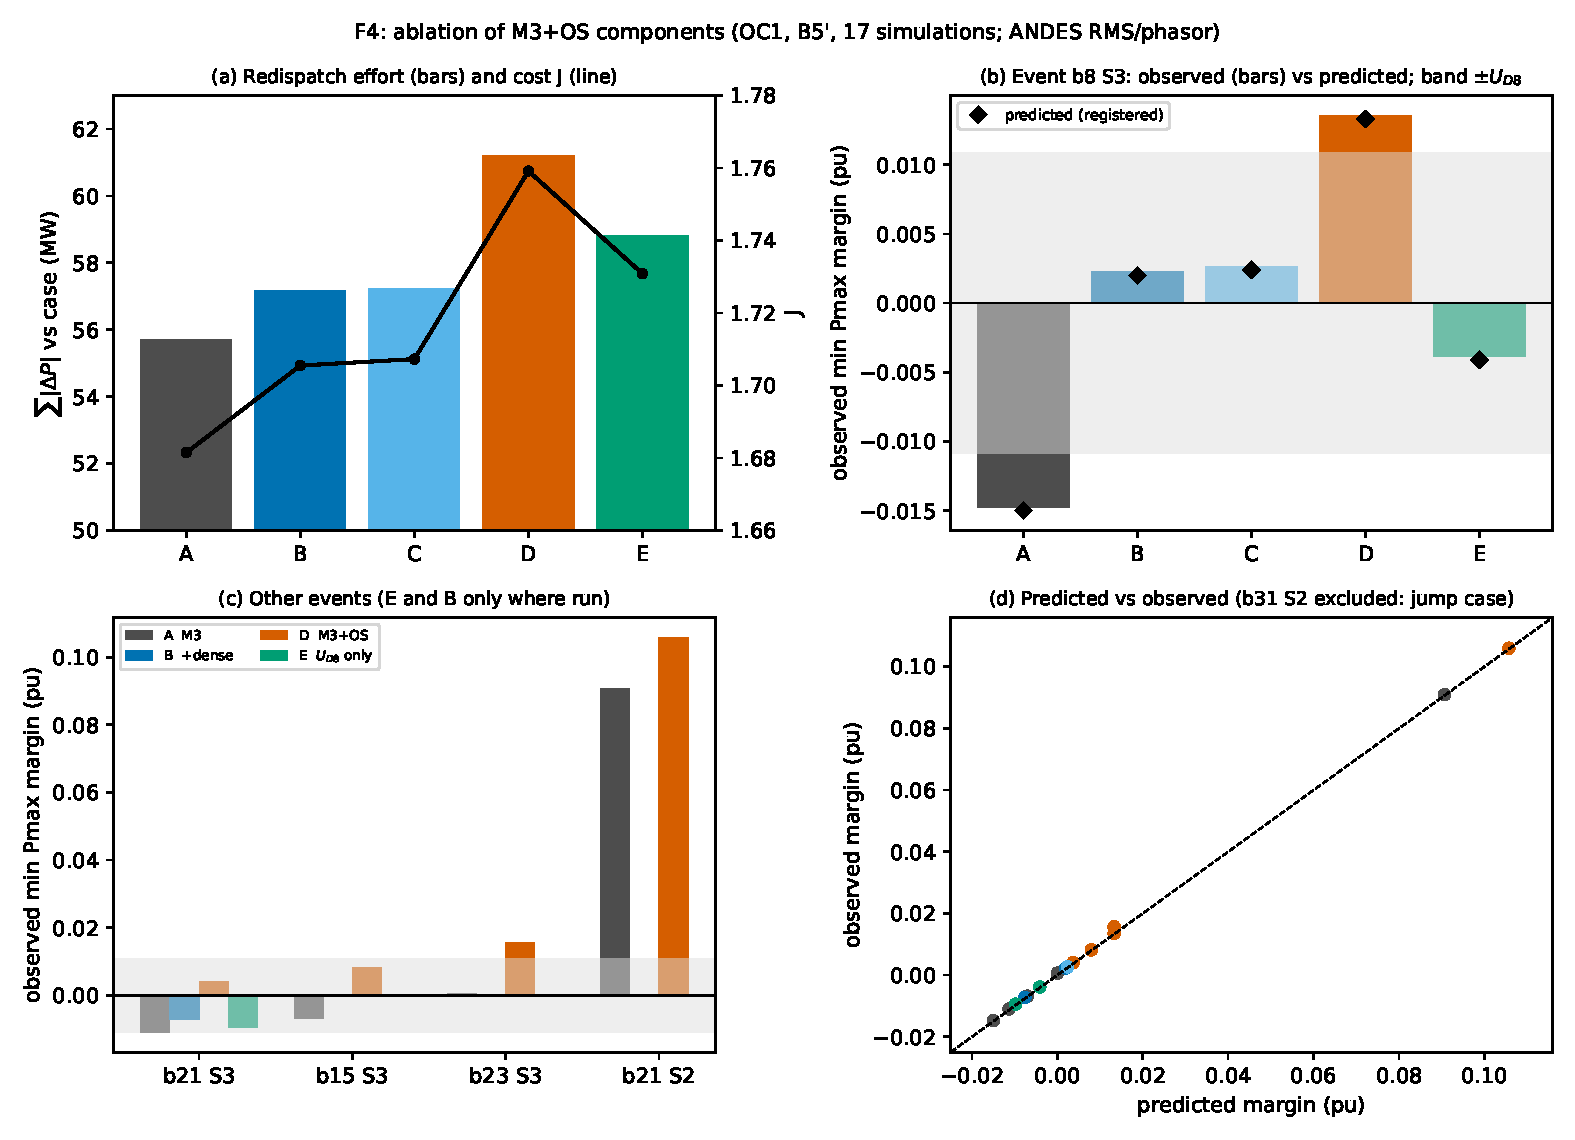
\includegraphics[width=\textwidth]{figures_main/DEC066_F4_final.pdf}
\caption{Ablation of the M3+OS components (OC1, B5$'$). (a) Redispatch effort and cost of the five designs. (b) Observed minimum Pmax margin at bus 8, S3 (bars) against the margin registered before the simulation (diamonds); the grey band is the numerical band $\pm U_{D8}$. (c) Observed margin at other events (designs not run in an event are omitted). (d) Predicted against observed margin for the 15 cells that are admissible at the jump. ANDES RMS/phasor results.}
\label{fig:f4}
\end{figure*}

\begin{figure*}[t]
\centering
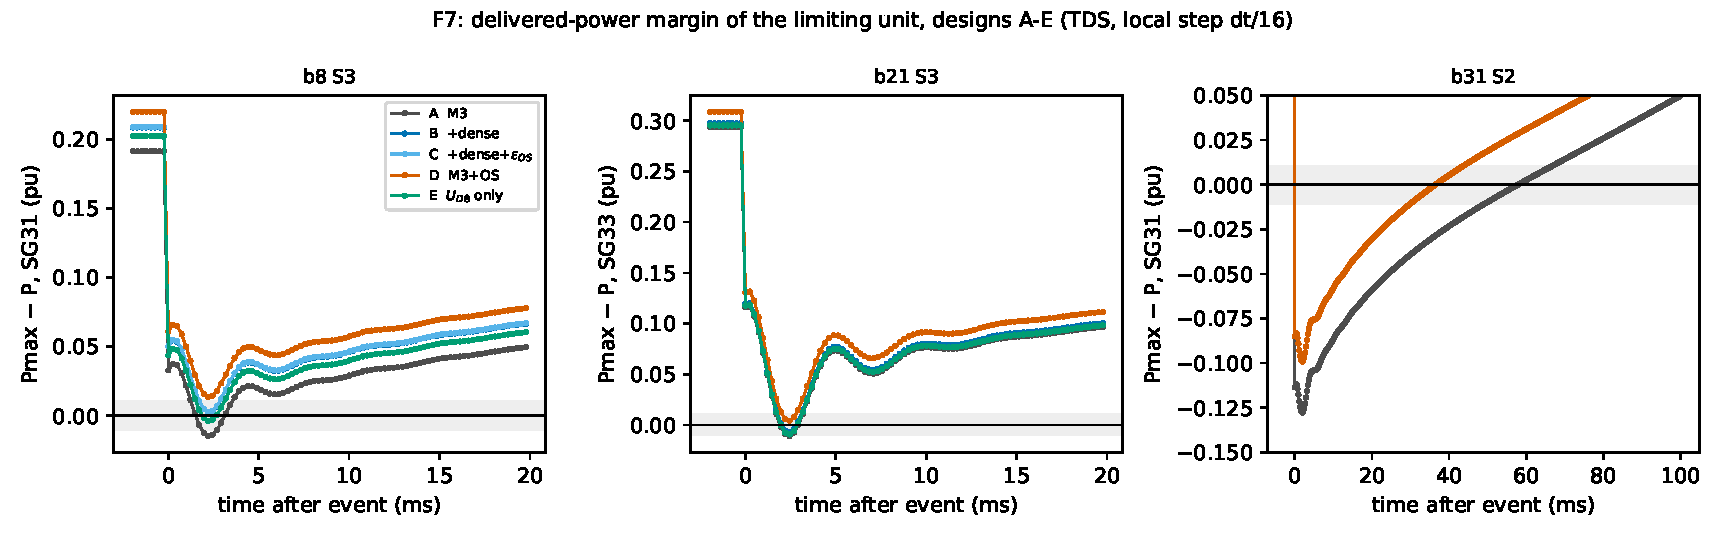
\includegraphics[width=\textwidth]{figures_main/DEC066_F7_transients.pdf}
\caption{Pmax margin of delivered power of the limiting unit for the five designs at bus 8, S3 (left), for A, B, D and E at bus 21, S3 (centre) and for A and D at bus 31, S2 (right, longer time scale). The pre-event headroom differs between designs; the minimum occurs about 2~ms after the event in the first two cases.}
\label{fig:f7}
\end{figure*}

\begin{figure*}[t]
\centering
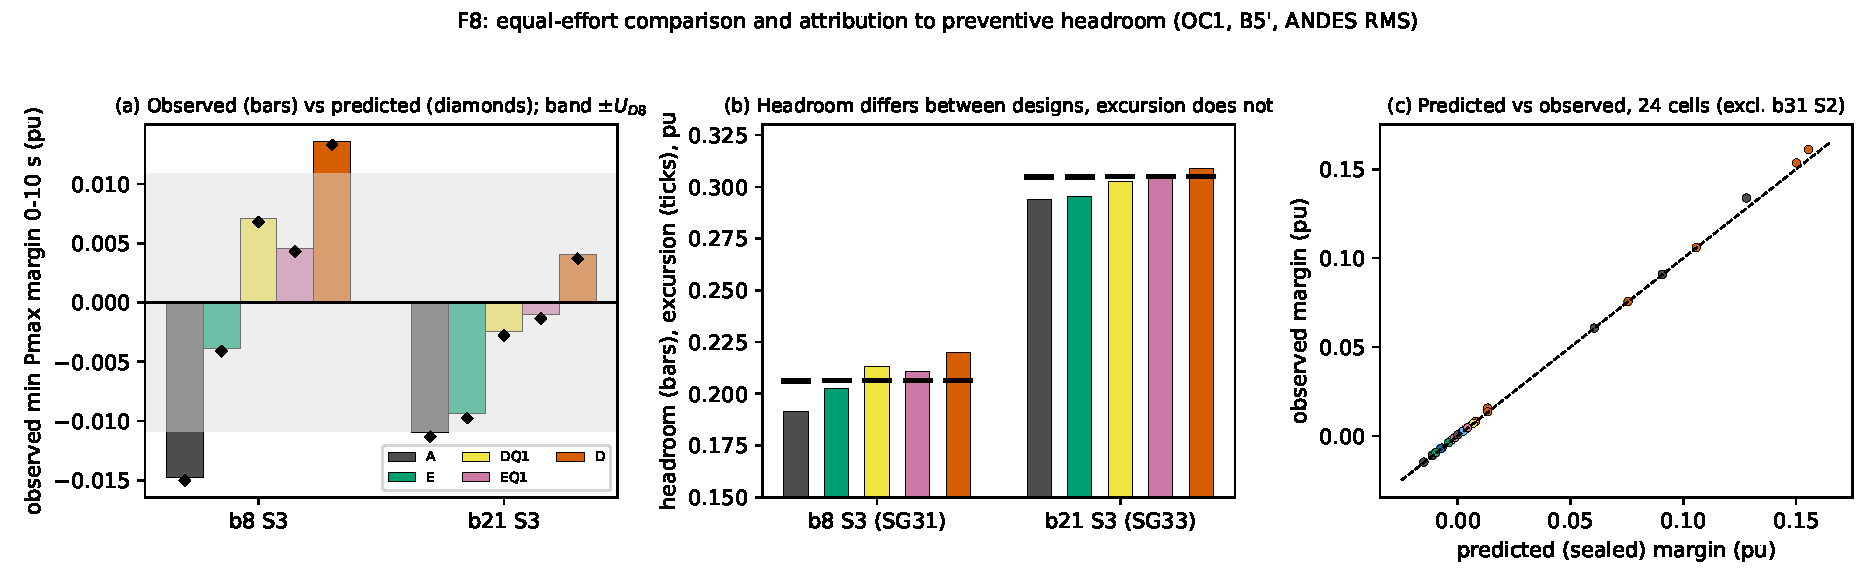
\includegraphics[width=\textwidth]{figures_main/DEC066_F8_equal_effort.pdf}
\caption{Equal-effort comparison (OC1, B5$'$, ANDES RMS). (a) Observed minimum Pmax margin 0--10~s (bars) and sealed prediction (diamonds) at bus 8 S3 and bus 21 S3 for A, E, DQ1 (effort of E, dense), EQ1 (effort of D, uniform band) and D; grey band $\pm U_{D8}$. (b) Pre-event headroom of the limiting unit (bars) and observed excursion (black ticks): the headroom differs between designs, the excursion does not. (c) Predicted against observed margin for the 24 cells admissible at the jump.}
\label{fig:f8}
\end{figure*}

\emph{Scope of this evidence.} The cells with the largest contrast, buses 8 and 23, are active constraints of the design and are therefore design-set (in-sample) for all variants; they show that the predicted constraint is reproduced, not that it generalises. Buses 21 and 15 were not design events (bus 21 was a blind bus of an earlier study, so its use here is retrospective), and bus 39 was observed before; only bus 18 is out-of-design and it is not discriminating. The equal-effort contrasts rest on two events at one operating condition. The effect is a few percent of Pmax, it acts within the first 3~ms, and its relevance for protection or equipment depends on a temporal tolerance of the limit that is not known; the results are RMS/phasor and do not support any statement about converter-level behaviour or about instantaneous physical protection.
